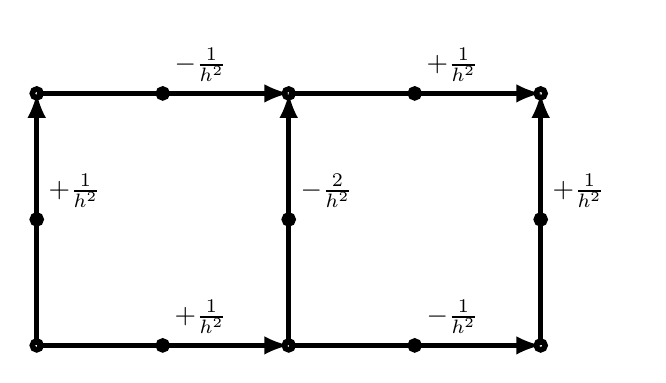
\begin{tikzpicture}[>=latex, line width=2pt, scale=0.8]

%define picture size
\draw[opacity=0] (-4.1,-2.1) rectangle (5.5,3);

\coordinate (V0) at (0,-2);
\coordinate (V1) at (4,-2);
\coordinate (V2) at (4,2);
\coordinate (V3) at (0,2);
\coordinate (V4) at (-4,2);
\coordinate (V5) at (-4,-2);

\coordinate (C0) at (0,0);
\coordinate (C1) at (2,-2);
\coordinate (C2) at (4,0);
\coordinate (C3) at (2,2);
\coordinate (C4) at (-2,2);
\coordinate (C5) at (-4,0);
\coordinate (C6) at (-2,-2);

\coordinate (CC0) at (-2,0);
\coordinate (CC1) at (2,0);

\draw (V0) circle(2pt);
\draw (V1) circle(2pt);
\draw (V2) circle(2pt);
\draw (V3) circle(2pt);
\draw (V4) circle(2pt);
\draw (V5) circle(2pt);


\draw (C1) node[above right]{$-\frac{1}{h^{2}}$} circle(2pt);
\draw (C2) node[above right]{$+\frac{1}{h^{2}}$} circle(2pt);
\draw (C3) node[above right]{$+\frac{1}{h^{2}}$} circle(2pt);
\draw (C4) node[above right]{$-\frac{1}{h^{2}}$} circle(2pt);
\draw (C5) node[above right]{$+\frac{1}{h^{2}}$} circle(2pt);
\draw (C6) node[above right]{$+\frac{1}{h^{2}}$} circle(2pt);

%\draw[gray] (CC0) circle(2pt);
%\draw[gray] (CC1) circle(2pt);

%\draw[->,gray] (CC1) -- (CC0);

%\draw[->,gray,densely dotted] (C2) -- (CC1);
%\draw[->,gray,densely dotted] (CC1) -- (C3);
%\draw[->,gray,densely dotted] (CC0) -- (C4);
%\draw[->,gray,densely dotted] (CC0) -- (C5);
%\draw[->,gray,densely dotted] (C6) -- (CC0);
%\draw[->,gray,densely dotted] (C1) -- (CC1);

\draw[->] (V0) -- (V3);
\draw[->] (V0) -- (V1);
\draw[->] (V1) -- (V2);
\draw[->] (V3) -- (V2);
\draw[->] (V4) -- (V3);
\draw[->] (V5) -- (V4);
\draw[->] (V5) -- (V0);

\draw (C0) node[above right]{$-\frac{2}{h^{2}}$} circle(2pt);


\end{tikzpicture}
